El objetivo de este curso es analizar las técnicas básicas para la \emph{transmisión digital de datos} sobre un canal imperfecto. Para ello, haremos un fuerte uso de las técnicas de análisis de señales en tiempo discreto y continuo (teoremas de muestreo, Transformada de Fourier, etc.), y las extenderemos para realizar modelos de transmisión adecuados a las señales digitales.

En primer lugar, corresponde definir nuestro objeto de trabajo:

\begin{definicion*}[Señal digital de tiempo discreto]
    Una \emph{señal digital} es una secuencia $\{a_k:k\in\mathbb{Z}\}$ de \emph{símbolos}, cada uno de ellos perteneciente a un \emph{alfabeto} finito:
    \begin{equation*}
        a_k \in \{s_1,\ldots,s_M\}
    \end{equation*} 
    siendo $M$ el tamaño del alfabeto.
\end{definicion*}

Cuando $M=2$, el alfabeto se denomina binario y cada símbolo puede interpretarse como un $0$ o un $1$, permitiendo así la transmisión básica de la información digital. Sin embargo, como veremos más adelante, puede ser relevante considerar alfabetos de mayor cantidad de símbolos, permitiendo enviar mayor cantidad de ``bits por símbolo'', es decir cada símbolo contiene una mayor cantidad de ``información''.

Notemos además que los símbolos no son necesariamente $0$ y $1$. Por ejemplo, para un alfabeto binario veremos que puede ser interesante codificar los símbolos como $1$ y $-1$ en algunas aplicaciones, de manera de obtener señales de valor medio nulo.

El objetivo entonces de un sistema de comunicación digital es transmitir, sobre un canal imperfecto, una señal digital de tiempo discreto y \emph{reconstruir}, a la salida, una señal digital $\{\hat{a}_k\}$ de manera tal de que \emph{maximizar la cantidad de símbolos reconstruidos de manera correcta}. Dicho de otro modo, si el sistema de transmisión, modulación, canal y detección introducen perturbaciones aleatorias, que la probabilidad de \emph{error de símbolo}, $\p{a_k\neq \hat{a}_k}$ sea (en régimen) la menor posible.

Como se intuye de la ecuación anterior, aparecen dos conceptos clave a tener en cuenta en el presente curso:

\begin{itemize}
    \item Es útil trabajar con \emph{señales aleatorias}. Esto es porque no conocemos a priori \emph{qué es lo que se va a transmitir}, y quizás solo propiedades estadísticas de la señal. A su vez, todo canal de comunicación está sujeto a \emph{ruido} que es intrínsecamente aleatorio. Esto requiere familiaridad con el concepto de \emph{proceso estocástico} que definiremos en el Capítulo \ref{chapter:procesos estocasticos}, así como con las reglas básicas de probabilidad, que se recuerdan en el Apéndice \ref{app:probabilidad}.
    
    \item Por otra parte, al tratarse de análisis de señales, tanto en tiempo discreto como tiempo continuo, se requiere familiaridad con los conceptos de sistemas lineales invariantes en el tiempo (que servirán para modelar el canal, entre otras cosas), así como la \emph{Transformada de Fourier}, tanto en su versión discreta como continua. En particular veremos cómo las propiedades estadísticas de una señal se relacionan, mediante la transformada de Fourier, con su \emph{densidad espectral de potencia}, concepto que definiremos también en el Capítulo \ref{chapter:procesos estocasticos}.
\end{itemize}

\section{Motivación de la transmisión digital}

La primera pregunta que debemos contestar es por qué puede ser conveniente transmitir datos de manera digital, esto es, siguiendo un alfabeto finito, en lugar de transmitir o intentar reproducir una forma de onda, como se vio en la modulación analógica. Si bien esta última fue el primer mecanismo masivo de transmisión de datos a larga distancia, y aún se utiliza hoy en múltiples aplicaciones (radio comercial, control de tráfico aéreo, etc.), debemos recordar que el \emph{primer sistema de transmisión eléctrica de datos} corresponde a la telegrafía: esto es, el envío de mensajes sobre un cable de cobre (cable telegráfico). Dichos mensajes correspondían típicamente a mensajes de texto (letras y números), que eran \emph{codificados} como pulsos de distinta duración (cortos y largos). Esto dio lugar al primer ejemplo de código para la transmisión eléctrica: el código Morse (1844, c.f. \href{https://en.wikipedia.org/wiki/Electrical_telegraph}{telégrafía eléctrica}).

\begin{figure}[h]
    \begin{center}
        \begin{tabular}{cc}
        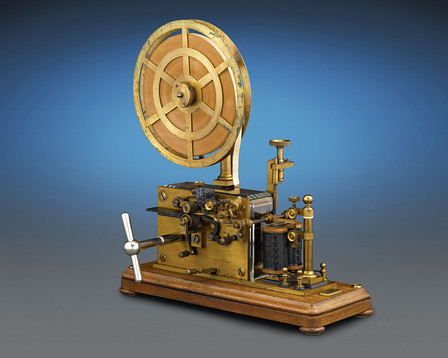
\includegraphics[margin=2em, width=0.4\textwidth]{figuras/Morse_Code_Receiver.png} &
        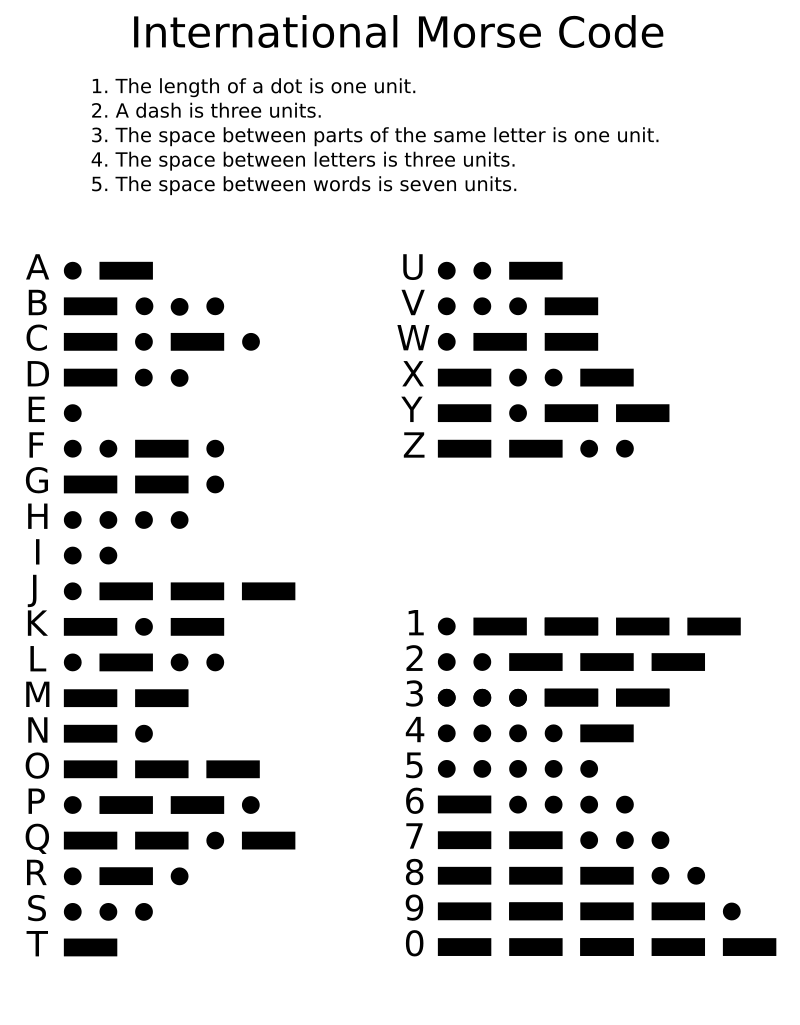
\includegraphics[margin=2em, width=0.3\textwidth]{figuras/International_Morse_Code.png}
        \end{tabular}
    \end{center}
    \caption{Telégrafo de Morse.}\label{fig:morse}
\end{figure}

Para entender las ventajas de la comunicación digital, es bueno remitirse primero a un esquema básico de comunicación analógico, como el mostrado en la Figura \ref{fig:analogico}. Allí, la fuente de información (ej. audio) es transformada en una señal eléctrica continua $x(t)$ por un transductor (ej. micrófono). El sistema de modulación intentará transmitir dicha señal por un medio físico, recibiendo $\hat{x}(t)$, señal que luego es enviada a otro transductor (ej. parlante) para enviarla al receptor. El objetivo de este proceso es que la señal $\hat{x}(t)$ reproduzca lo más fielmente posible la señal original $x(t)$, en todo momento del tiempo. Sin embargo, esto resulta imposible debido a que el canal siempre introduce atenuación, limitaciones de ancho de banda, potencia de transmisión y ruido que alteran la recepción (en algunos casos hasta volverla inservible).

En la transmisión digital, se transmiten símbolos $a_k$ construyendo una señal real $x(t)$ que depende de dichos símbolos. Si la señal recibida $\hat{x}(t)$ es suficientemente inteligible, podemos decodificar el símbolo $\hat{a}_k$ con \emph{muy  alta probabilidad} de que sea exactamente igual a $a_k$. En ese caso, la reconstrucción de la señal es perfecta (con alta probabilidad). Es decir, \emph{no hay pérdida de información por atravesar el canal}. Esto vuelve la transmisión mucho más robusta al ruido e interferencia. El objetivo principal de este curso es entender precisamente cómo realizar este proceso.

\begin{figure}
    \begin{center}
        
        \begin{blockdiagram}
        \node [block] (fuente) {Fuente};
        \node [block, right = of fuente] (transducer) {Transductor};
        \node [block, right = 6em of transducer] (tx) {Transmisor};
        \node [block, below = of tx] (ch) {Canal};
        \node [block, below = of ch] (rx) {Receptor};
        \node [block, left = 6em of rx] (transducer2) {Transductor};
        \node [block, left = of transducer2] (sink) {Receptor};
        \draw[thick, ->] (fuente)--(transducer);
        \draw[thick, ->] (transducer)--node[midway, above] {$x(t)$} (tx);
        \draw[thick, ->] (tx)--(ch);
        \draw[thick, ->] (ch)--(rx);
        \draw[thick, ->] (rx)--node[midway, above] {$\hat{x}(t)$} (transducer2);
        \draw[thick, ->] (transducer2)--(sink);
        \begin{scope}[on background layer]
            \node[draw, rectangle, dashed, fill=gray!25!white, fit=(tx) (ch) (rx), inner sep=10pt, label=below:Moduladción analógica] (modulador) {};
        \end{scope}

        \end{blockdiagram}
        \caption{Diagrama general de un sistema de transmisión analógico.}\label{fig:analogico}
    \end{center}
\end{figure}

Complementario a lo anterior existen dos fuertes razones para analizar la transmisión digital de datos:
\begin{enumerate}
    \item En primer lugar, en los últimos años, casi toda la información se almacena en forma digital (texto, fotos, video). En ese sentido, la información ya se encuentra en un alfabeto de símbolos (ej. binario) y no tiene sentido plantearse pasar por una etapa analógica, salvo para efectivamente transmitir sobre el medio físico.
    
    \item En otros casos, la señal analógica se convierte en una señal digital mediante un conversor analógico/digital (A/D) (Figura \ref{fig:a/d}) Aquí se cumplen dos etapas:
     \begin{enumerate}
        \item Se \emph{muestrea la señal} a una frecuencia de muestreo $f_s$ (muestras por segundo).
        \item Se \emph{cuantifica la señal} pasando el valor analógico a una cierta cantidad de símbolos (bits). Por ejemplo, las señales de audio se muestrean a $f_s=44100 \unit{Hz}$ y se digitalizan utilizando $16$ bits de resolución para cada canal estéreo. El resultado es una secuencia de muestras $a_k$ de $\approx 1.41 \unit{\mega bps}$.
     \end{enumerate}
\end{enumerate}

\begin{figure}
    \begin{center}        
        \begin{blockdiagram}
        \node [block, align=center] (fuente) {Fuente \\ analógica};
        \node [block, right = 5em of fuente, align=center, label=below:{Frec: $f_s$, $N$ bits}] (ad) {Conversor \\ A/D};
        \node [right = 5em of ad] (salida) {$Nf_s \unit{bps}$};
        \draw[thick, ->] (fuente)--node[midway,above] {$x(t)$} (ad);
        \draw[thick, ->] (ad)--node[midway, above] {$a_k$} (salida);
        \end{blockdiagram}
        \caption{Conversión analógica a digital.}\label{fig:a/d}
    \end{center}
\end{figure}

En el segundo caso, por el Teorema de Nyquist del muestreo, sabemos que si la señal $x(t)$ tiene ancho de banda $B$, entonces obteniendo muestras a frecuencia $f_s>2B$ es posible reconstruir la señal de manera \emph{exacta} a partir de las muestras $x(kT_s)$ con $T_s=1/f_s$. Sin embargo, como las muestras están cuantificadas, $a_k\approx x(kT_s)$ pero no es exacto, introduciendo el llamado \emph{ruido de cuantificación}. Este ruido es menor a mayor cantidad de bits utilizados para representar las muestras. Sin embargo, si la transmisión digital permite reconstruir las muestras $a_k$ exactamente, es probable que dicho ruido de cuantificación sea menor que el que introduce un esquema de modulación analógico, por lo cual la señal se recibe de mejor manera. A su vez, con los esquemas de modulación modernos, es posible aprovechar mejor el ancho de banda mandando más información (bits) sobre el mismo, por lo cual podemos realizar transmisiones de calidad.

\section{Diagrama general de un sistema de transmisión digital}

El diagrama general de un sistema de transmisión digital se muestra en la Figura \ref{fig:digital}. Allí partimos de una fuente ya digital que genera símbolos $\{a_k\}$, y se pasa por dos etapas de codificación que explicaremos. Con ello se genera una nueva señal digital $\{b_k\}$ que se enviará por el medio físico. Para ello, se requiere una etapa de \emph{modulación digital}, en la cual los símbolos $b_k$ se convierten en una señal analógica adecuada, se envían por el canal, y luego son reconstruidos por un \emph{detector} digital, que obtiene una secuencia $\hat{b}_k$. El objetivo de esta etapa es lograr que $\p{\hat{b}_k=b_k}$ sea máxima, de este modo permitiendo reconstruir la señal. Luego esta se decodifica por el proceso inverso a la codificación para obtener $\hat{a}_k$ y enviar esta señal al receptor. 

\begin{figure}
    \begin{center}
        
        \begin{blockdiagram}[node distance=3em]
        \node [block,align=center] (fuente) {Fuente \\ digital};
        \node [block, right = 5em of fuente, align=center] (codfuente) {Cod. de fuente};
        \node [block, right = of codfuente, align=center] (codcanal) {Cod. de canal};
        \node [block, right = 5em of codcanal] (tx) {Transmisor};
        \node [block, below = of tx] (ch) {Canal};
        \node [block, below = of ch] (rx) {Receptor};
        \node [block, left = 5em of rx] (decocanal) {Decod. canal};
        \node [block, left = of decocanal] (decofuente) {Decod. fuente};
        \node [block, left = 5em of decofuente, align=center] (sink) {Receptor \\ digital};

        \draw[thick, ->] (fuente)--node[midway,above] {$a_k$} (codfuente);
        \draw[thick, ->] (codfuente)--(codcanal);
        \draw[thick, ->] (codcanal)--node[midway,above] {$b_k$} (tx);
        \draw[thick, ->] (tx)--node[midway,right] {$x(t)$} (ch);
        \draw[thick, ->] (ch)--node[midway,right] {$\hat{x}(t)$} (rx);
        \draw[thick, ->] (rx)--node[midway,above] {$\hat{b}_k$} (decocanal);
        \draw[thick, ->] (decocanal)--(decofuente);
        \draw[thick, ->] (decofuente)--node[midway,above] {$\hat{a}_k$} (sink);
        
        \node [block, right = of ch] (sinc) {Sincronismo};
        \draw[thick, -] (tx) -| (sinc);
        \draw[thick, ->] (sinc) |- (rx);

        \begin{scope}[on background layer]
            \node[draw, rectangle, dashed, fill=gray!25!white, fit=(tx) (ch) (rx) (sinc), inner sep=10pt, label=below:Moduladción digital] (modulador) {};
            \node[draw, rectangle, dashed, fill=gray!25!white, fit=(codfuente) (codcanal), inner sep=10pt, label=below:Etapa de codificación] (cod) {};
            \node[draw, rectangle, dashed, fill=gray!25!white, fit=(decofuente) (decocanal), inner sep=10pt, label=below:Etapa de decodificación] (decod) {};

        \end{scope}
        \end{blockdiagram}

        \caption{Diagrama general de un sistema de transmisión digital.}\label{fig:digital}
    \end{center}
\end{figure}

El objetivo de este curso es analizar la etapa de \emph{modulación digital}, es decir dada una secuencia de símbolos $\{b_k\}$, cómo construir una señal analógica $x(t)$ que contenga la información de dichos símbolos y sea adecuada para su transmisión por el medio físico (radio, par de cobre, fibra óptica). Luego de su transmisión, la señal alterada deberá ser detectada y de allí reconstruiremos una secuencia de símbolos con baja probabilidad de error. El término modulación digital hace referencia a que la señal discreta \emph{modula} características de la señal analógica. Notemos además que este proceso requiere un bloque adicional: el \emph{sincronismo}, para que el receptor sepa a qué velocidad se transmite la información y cuál es el mejor momento del tiempo para muestrear la señal $\hat{x}(t)$ de manera de recuperar $\hat{b}_k$.

Si bien en este curso no trabajaremos sobre la etapa de \emph{codificación}, es importante entender el rol que cumplen las mismas previo a la transmisión. Introducimos ahora los principales conceptos.

\section{Conceptos básicos de codificación}

Como se observa en la Figura \ref{fig:digital}, existen dos etapas: la \emph{codificación de fuente} y la \emph{codificación de canal}, con sus respectivos decodificadores.

\subsection{Codificación de fuente}

El objetivo de la codificación de fuente es \emph{eliminar redundancia} de los datos, produciendo una secuencia de símbolos con menor cantidad de ``bits por símbolo'', de manera de requerir menor velocidad de transmisión de información. Existen dos tipos:
\begin{description}
    \item[Codificación sin pérdida:] Aquí la secuencia de símbolos generada contiene toda la información de la señal $\{a_k\}$, pero \emph{comprimida}. Esto es, utilizando propiedades estadísticas de la señal, se logra representar la misma información con menos bits. Un ejemplo de esto es el algoritmo \href{https://en.wikipedia.org/wiki/LZ77_and_LZ78}{Lempel-Ziv}, utilizado en la compresión ``.zip''.
    
    \item[Codificación con pérdida:] Aquí la secuencia de símbolos generada contiene \emph{menos información} que la original, eliminando por ejemplo partes que no son requeridas por el receptor. Ejemplos de esto son la compresión de imágenes JPEG, la compresión de video MPEG y la codificación de audio MP3. En estos casos, la señal reconstruida es una ``buena aproximación'' de la información original. Qué quiere decir ``buena aproximación'' depende de la aplicación, pero a modo de ejemplo el MP3 permite reducir la velocidad de audio mencionada anteriormente ($1.41 \unit{\mega bps}$) a $192 \unit{\kilo bps}$ o menos sin que el usuario detecte mayormente la diferencia. 
\end{description}

\begin{ejemplo}[Codificación sin pérdida]\label{ej:lossless}
Consideremos una fuente de datos que genera símbolos \emph{independientes} con la siguiente estadística:
\begin{equation*}
    a_k \in \{0,1,2,3\} \text{ con distribución } \begin{cases}
    \p{a_k=0} = 1/2 \\
    \p{a_k=1} = 1/4 \\
    \p{a_k=2} = 1/8 \\
    \p{a_k=3} = 1/8 \\
    \end{cases}
\end{equation*}
En este caso, una codificación sencilla sería tomar el código:
\begin{equation*}
    \begin{cases}
        a_k = 0 \mapsto \tilde{a}_k = 00 \\
        a_k = 1 \mapsto \tilde{a}_k = 01 \\
        a_k = 2 \mapsto \tilde{a}_k = 10 \\
        a_k = 3 \mapsto \tilde{a}_k = 11 \\
    \end{cases}
\end{equation*}
Observemos que el código anterior requiere en promedio 2 bits por símbolo (ya que todos los códigos son de 2 bits). ¿Podemos hacerlo mejor? Consideremos el siguiente código, debido a \href{https://en.wikipedia.org/wiki/Huffman_coding}{Huffman}:
\begin{equation*}
    \begin{cases}
        a_k = 0 \mapsto \tilde{a}_k = 0 \\
        a_k = 1 \mapsto \tilde{a}_k = 10 \\
        a_k = 2 \mapsto \tilde{a}_k = 110 \\
        a_k = 3 \mapsto \tilde{a}_k = 111 \\
    \end{cases}
\end{equation*}

Notemos que el código anterior es un \emph{código de prefijo} (cada símbolo empieza de manera diferente), lo que permite que sea invertible. Es decir si por ejemplo recibimos:
\begin{equation*}
    0101001110110111 \mapsto 0\;10\;10\;0\;111\;0\;110\;111 \mapsto 01103023
\end{equation*}
Calculemos el largo medio de la palabra enviada de la siguiente forma, donde $\ell(\cdot)$ representa el largo del código:
\begin{align*}
    \bar{L} &= \p{a_k=0} \ell(0) + \p{a_k=1} \ell(10) + \p{a_k=2} \ell(110) + \p{a_k=3} \ell(111)\\
    &= \left(\frac{1}{2}\right)(1) + \left(\frac{1}{4}\right)(2) + \left(\frac{1}{8}\right)(3) + \left(\frac{1}{8}\right)(3) = 1.75 < 2
\end{align*}

Esto quiere decir que en el largo plazo, una secuencia de $N$ símbolos podrá ser representada por $\approx 1.75 N$ bits (en lugar de $2N$), permitiendo un ahorro.
\end{ejemplo}

La clave del ejemplo anterior está en elegir palabras más largas para símbolos menos frecuentes. Notemos que esto mismo ya había sido advertido por Morse en su código, como se ve en la Figura \ref{fig:morse}. Surgen entonces las siguientes preguntas: ¿cuál es el mínimo largo medio posible de codificación? ¿Es alcanzable?

En 1948, \href{https://en.wikipedia.org/wiki/Claude_Shannon}{Claude Shannon} establece la teoría matemática de transmisión de información, introduciendo el concepto de \emph{entropía} de una fuente. Dicha entropía representa la cantidad de información contenida en una fuente (considerando sus propiedades estadísticas). Para una fuente $X$ que genera símbolos independientes $\{a_k\}$, la misma se define como:
\begin{equation*}
    H(X) = -\sum_k p_k \log_2(p_k)
\end{equation*}
siendo $p_k$ la probabilidad de cada símbolo y $\log_2$ el logaritmo en base $2$, lo que hace que la entropía quede en bits/símbolo.

Calculemos la entropía de la fuente anterior:
\begin{equation*}
    H(X) = \left(\frac{1}{2}\right)(1) + \left(\frac{1}{4}\right)(2) + \left(\frac{1}{8}\right)(3) + \left(\frac{1}{8}\right)(3) = 1.75.
\end{equation*}
Es decir, recuperamos exactamente el largo medio del código de Huffman anterior.

\begin{ejemplo}[Fuente binaria]\label{ej:entropia binaria}
    Supongamos que los símbolos son binarios $a_k\in\{0,1\}$ con $\p{a_k=1} = p = 1-\p{a_k=0}$ e independientes. En ese caso la entropía queda (como función de $p$):
    \begin{equation}\label{eq:entropia binaria}
        H(p) = -p\log_2 (p) - (1-p) \log_2(1-p),
    \end{equation}
    cuya gráfica puede verse en la Figura \ref{fig:entropia binaria}.
\end{ejemplo}


\begin{figure}
    \begin{center}
        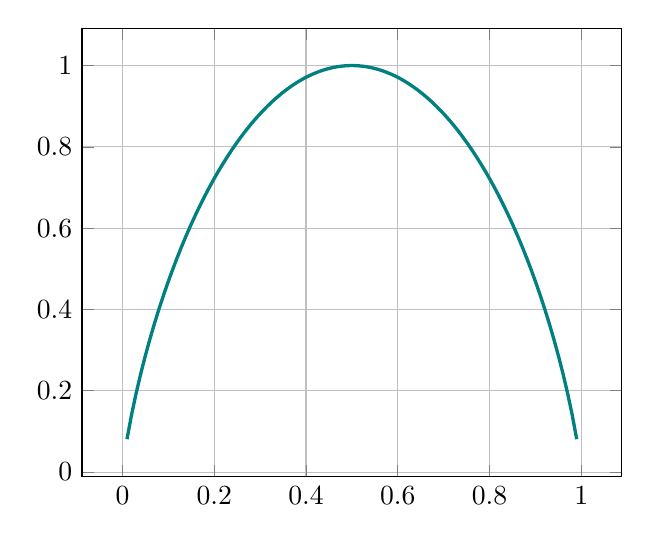
\begin{tikzpicture}
            \begin{axis}[grid]
            \addplot[domain=0.01:.99,samples=100, color=teal, very thick] {-x*ln(x)/ln(2) - (1-x)*ln(1-x)/ln(2)};
            \end{axis}
        \end{tikzpicture}
    \end{center}
    \caption{Entropía de una fuente binaria. Notar que el máximo se alcanza para $p=1/2$, es decir, distribución uniforme.}\label{fig:entropia binaria}
\end{figure}

El Teorema de Shannon muestra que para una fuente dada, su entropía es la mínima cantidad de bits por símbolo alcanzable:
\begin{teorema}[Shannon, 1948]
Sea una fuente de símbolos $\{a_k\}$ y su entropía $H_a$. Entonces es posible agrupar los símbolos de a bloques de tamaño $N$ y codificarlos en palabras de $L_N$ bits de manera que el largo medio de palabra cumpla:
\begin{equation*}
    N H_a \leqslant \bar{L}_N \leqslant NH_a + 1 
\end{equation*}
Como cada bloque codifica $N$ símbolos, la cantidad de bits por símbolo será entonces:
\begin{equation*}
    H_a \leqslant \frac{\bar{L}}{N} \leqslant H_a + 1/N
\end{equation*}
Además, no existe ningún código que logre mejorar esta cota.
\end{teorema}

La entropía de una fuente nos entonces da la mínima cantidad de bits por símbolo que podemos utilizar, es decir, el límite de la compresión alcanzable. Si volvemos al Ejemplo \ref{ej:lossless}, vemos que precisamente el código de Huffman alcanza la mínima entropía posible, incluso con $N=1$. Para otras distribuciones puede ser necesario utilizar un largo mayor de bloque para aproximar la entropía.

En el Ejemplo \ref{ej:entropia binaria}, vemos que la entropía es máxima e igual a $1$ cuando los símbolos son \emph{equiprobables} ($p=1/2$). En ese caso, debemos utilizar 1 bit por símbolo y la señal es incompresible. Precisamente, el código de Huffman descrito logra que la fuente original genere cantidades equiprobables de $0$ y $1$, por lo cual no puede comprimirse más.

Si en cambio $p\to 0$, la fuente tiene secuencias largas de $0$, y en ese caso puede ser más eficiente codificar el largo de la cadena de $0$s que indicar cada bit por separado. En el caso extremo, solo alcanza 1 bit para toda la cadena (``son todos ceros''). Análogamente, si $p\to 1$.

\subsection{Codificación de canal}

El objetivo de la codificación de fuente es reducir la cantidad de datos a transmitir a su mínima expresión, eliminando redundancia sin pérdida de información (o en el caso con pérdida, sin distorsión relevante). La \emph{codificación de canal} va en sentido opuesto: agrega redundancia para anticiparse a posibles errores del canal de transmisión y poder detectarlos y corregirlos. A continuación damos algunos ejemplos.

\begin{ejemplo}[Bit de paridad]\label{ej:paridad}
    Supongamos una fuente binaria $\{a_k\}$ y formemos bloques de largo $N$. Al final de cada bloque se agrega un bit $a_N = a_0 \oplus \ldots \oplus a_{N-1}$ donde $\oplus$ es la operación XOR. Luego se transmite la palabra $b = (a_0,\ldots,a_N)$. El resultado final es que $a_N=1$ si hay una cantidad impar de $1$s en el bloque, o dicho de otro modo, cada bloque $b$ tiene una cantidad par de bits. Esto permite \emph{detectar} (pero no corregir) errores de $1$ bit, con un overhead de $1/N$ bits por símbolo.

    Obviamente, si el largo de bloque $N$ es grande, el overhead es mínimo, pero la probabilidad de que haya errores de más de un bit es mayor, por lo cual la elección de $N$ es un compromiso entre ambos efectos.
\end{ejemplo}

\begin{ejemplo}[Código de repetición]\label{ej:codrep}
    Supongamos una fuente binaria $\{a_k\}$ y realicemos el siguiente procedimiento: para cada símbolo $a_k$ formamos un bloque $b=(a_k, a_k, a_k)$. Esto es un código de repetición de largo $3$. Observemos que si hay un error de $1$ bit, podemos decidir por mayoría si el bloque corresponde a un $0$ o a un $1$. Por ejemplo $(110)\mapsto 1$ y $(010)\mapsto 0$. Esto permite \emph{detectar y corregir} errores de $1$ bit. Sin embargo, requiere 3 bits por símbolo, lo cual es ineficiente.
\end{ejemplo}

\begin{ejemplo}[Matriz de paridad]\label{ej:parity matrix}
    Consideremos ahora el siguiente procedimiento para una fuente binaria $\{a_k\}$. Elegimos un número $M$ y formamos bloques de tamaño $N=M^2$ dispuestos en forma de matriz de $M\times M$. Luego se agrega a dicha matriz un bit de paridad para cada fila y cada columna, así como un bit de paridad total. Por ejemplo, si $M=4$, $N=16$:
    \begin{equation*}
        (1001000111111011) \; \mapsto\; \begin{pmatrix}
            1 & 0 & 0 & 1 \\
            0 & 0 & 0 & 1 \\
            1 & 1 & 1 & 1 \\
            1 & 0 & 1 & 1 \\
        \end{pmatrix} \; \mapsto \; \begin{pmatrix}
            1 & 0 & 0 & 1 & \vdots & 0 \\
            0 & 0 & 0 & 1 & \vdots & 1 \\
            1 & 1 & 1 & 1 & \vdots & 0 \\
            1 & 0 & 1 & 1 & \vdots & 1 \\
            \cdots & \cdots & \cdots & \cdots & \cdots & \cdots \\
            1 & 1 & 0 & 0 & \vdots & 0 \\
        \end{pmatrix}
    \end{equation*}
    Luego se envían los $N$ bits y los $M+1$ bits de paridad agregados.

    Si hay un error de un bit, el mismo se \emph{detecta} y se \emph{corrige} porque los errores de paridad indican la fila y columna del error, por ejemplo:
    \begin{equation*}
         \begin{pmatrix}
            1 & 0 & 0 & 1 & \vdots & 0 \\
            0 & 0 & 0 & 1 & \vdots & 1 \\
            1 & 1 & 1 & 1 & \vdots & 0 \\
            1 & 0 & 1 & 1 & \vdots & 1 \\
            \cdots & \cdots & \cdots & \cdots & \cdots & \cdots \\
            1 & 1 & 0 & 0 & \vdots & 0 \\
        \end{pmatrix} \; \rightsquigarrow  \;
         \begin{pmatrix}
            1 & 0 & 0 & 1 & \vdots & 0 \\
            0 & 0 & {\color{red} 1} & 1 & \vdots & 1{\color{red} *} \\
            1 & 1 & 1 & 1 & \vdots & 0 \\
            1 & 0 & 1 & 1 & \vdots & 1 \\
            \cdots & \cdots & \cdots & \cdots & \cdots & \cdots \\
            1 & 1 & 0{\color{red} *} & 0 & \vdots & 0 \\
        \end{pmatrix}
    \end{equation*}
    El código detecta entonces donde ocurrió el error porque la paridad de la fila y la columna no es correcto. Notar que el error también puede ocurrir en la fila o en la columna de paridad. Esto también se detecta y se corrige gracias al bit extra de paridad total.

    El resultado es que se envían $N$ bits con una redundancia de $2M+1 = 2\sqrt{N} + 1$ por lo que en un bloque de $N=1024$ bits solo se requieren $65$ bits extra. El overhead crece más lento que el tamaño de bloque. De todos modos sigue siendo ineficiente y solo permite corregir errores de $1$ bit, por lo que si el tamaño de bloque es grande, tenemos el mismo problema que en Ejemplo \ref{ej:paridad}.
\end{ejemplo}

El punto común de todos los ejemplos anteriores es el siguiente: dado un alfabeto de símbolos (por ejemplo binario), construimos bloques de largo $N$. Esto permite generar $2^N$ símbolos posibles. Luego agregamos bits de control, generando palabras de largo $N+r$, y aplicando un código que lleva secuencias de largo $N$ a un \emph{espacio mayor} de largo $N+r$, donde los códigos ``válidos'' se encuentran \emph{más separados entre sí} (solo hay $2^N$ palabras válidas de las $2^{N+r}$ posibles). Cuando ocurre algún error, encontramos una palabra no válida y detectamos el error. Si el código es adecuado, podemos además mapear esa palabra no válida a un símbolo válido ``cercano'' corrigiendo entonces el error.

A mayor $r$, más redundancia se agrega, más espacio se genera, y podemos detectar y corregir errores más grandes. Pero por otra parte, el overhead es mayor. Se le denomina \emph{tasa de codificación (code rate)} al cociente $N/(N+r)$.

Un ejemplo de código de este tipo son los \href{https://en.wikipedia.org/wiki/Hamming_code}{Códigos de Hamming}, en los cuales se elige un tamaño de bloque $N+r=2^{r}-1$ con $r\geqslant 1$ y se envía un mensaje de largo $N=2^{r} - r - 1$ con $r$ bits de redundancia, utilizando una transformación lineal invertible. En ese caso, la tasa de codificación queda:
\begin{equation*}
    R = 1-\frac{r}{2^r-1},
\end{equation*}
es decir, la redundancia es del orden de $\log_2(N)\ll \sqrt{N}$. Sin embargo, si bien es más eficiente que la matriz de paridad, este código solo permite detectar errores de 1 o 2 bits, y corregir errores de un único bit. El tipo más común de código de bloques es el de \href{https://en.wikipedia.org/wiki/Reed\%E2\%80\%93Solomon_error_correction}{Reed--Solomon, 1960}, una familia de códigos que permite detectar errores de hasta $r$ bits y corregir hasta $\lfloor r/2 \rfloor$ bits, siendo $r$ un parámetro, la cantidad de redundancia deseada. Es además capaz de recuperar errores de ``borrado'', donde no es posible decidir si el bit recibido es $0$ o $1$.

Más recientemente, la aparición de los \href{https://en.wikipedia.org/wiki/Convolutional_code}{códigos convolucionales}, \href{https://en.wikipedia.org/wiki/Turbo_code}{Turbo--codes} y códigos \href{https://en.wikipedia.org/wiki/Low-density_parity-check_code}{Low--Parity--Data--Check}, se logran tasas de codificación cercanas a $1$ con muy baja probabilidad de error. 

